\documentclass{beamer}
\usetheme[faculty=law]{fibeamer}
\usepackage[utf8]{inputenc}
\usepackage[main=english]{babel}
\title{Cancer Detection} %% that will be typeset on the
\subtitle{An introduction to cancer detection using deep learning} %% title page.
\author{Mahdi Lotfi \\ Erfan Momeni \\ Araz Abedini \\ Matin Ghanbari}
%% These additional packages are used within the document:
\usepackage{ragged2e}  % `\justifying` text
\usepackage{booktabs}  % Tables
\usepackage{tabularx}
\usepackage{tikz}      % Diagram
\usetikzlibrary{calc, shapes, backgrounds}
\usepackage{epigraph}
\usepackage{amsmath, amssymb}
\usepackage{url}       % `\url`s
\usepackage{listings}  % Code listing
\begin{document}
  % \shorthandoff{-}
  \frame[c]{\maketitle}
  \AtBeginSection[]{% Printt an outline at the beginning of sections
    \begin{frame}<beamer>
      \frametitle{Outline for Section \thesection}
      \tableofcontents[currentsection]
    \end{frame}}

    \section{Machine Learning}
    \subsection{What Is Machine Learning}
    \begin{frame}[t]{Machine Learning}
      \framesubtitle{a glance}%
      \begin{tikzpicture}[overlay,remember picture]
        \node[anchor=south east,xshift=-30pt,yshift=35pt]
          at (current page.south east) {
            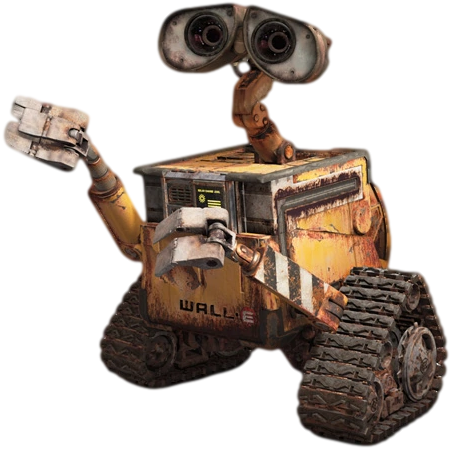
\includegraphics[width=35mm]{resources/wall-e}
          };
      \end{tikzpicture}%
      \begin{quote}
        field of study that gives computers the ability to learn without being explicitly programmed.
        \hfill {\tiny —Arthur Samuel, 1959}
      \end{quote}
      Machine Learning is the science (and art) of programming computers so they can \textit{learn from data}. \\
      \vspace{8mm}
      \parbox{0.55\textwidth}{
      Your spam filter is a Machine Learning program that, given examples of spam emails and examples of regular emails, can learn to flag spam.
      }
    \end{frame}
    \subsection{Types of Learning}
    \begin{frame}[label=lists]{Types of Machine Learning Systems}
      There are four types of machine learning algorithms:
      \newline
      \begin{columns}[onlytextwidth]
        \column{.7\textwidth}
          \begin{itemize}
            \item Supervised Machine Learning
            \item Unsupervised Machine Learning
            \item Semi-Supervised Machine Learning
            \item Reinforcement Learning
            \end{itemize}
      \end{columns}
      
    \end{frame} 
    
    \begin{frame}[t]{Supervised Machine Learning}
      \justifying It is based on training data. we train the machines using the "labeled" dataset, and based on the training, the machine predicts the output. 
    
      \begin{tikzpicture}[overlay,remember picture]
        \node[anchor=south east,xshift=-20pt,yshift=30pt]
          at (current page.south east) {
            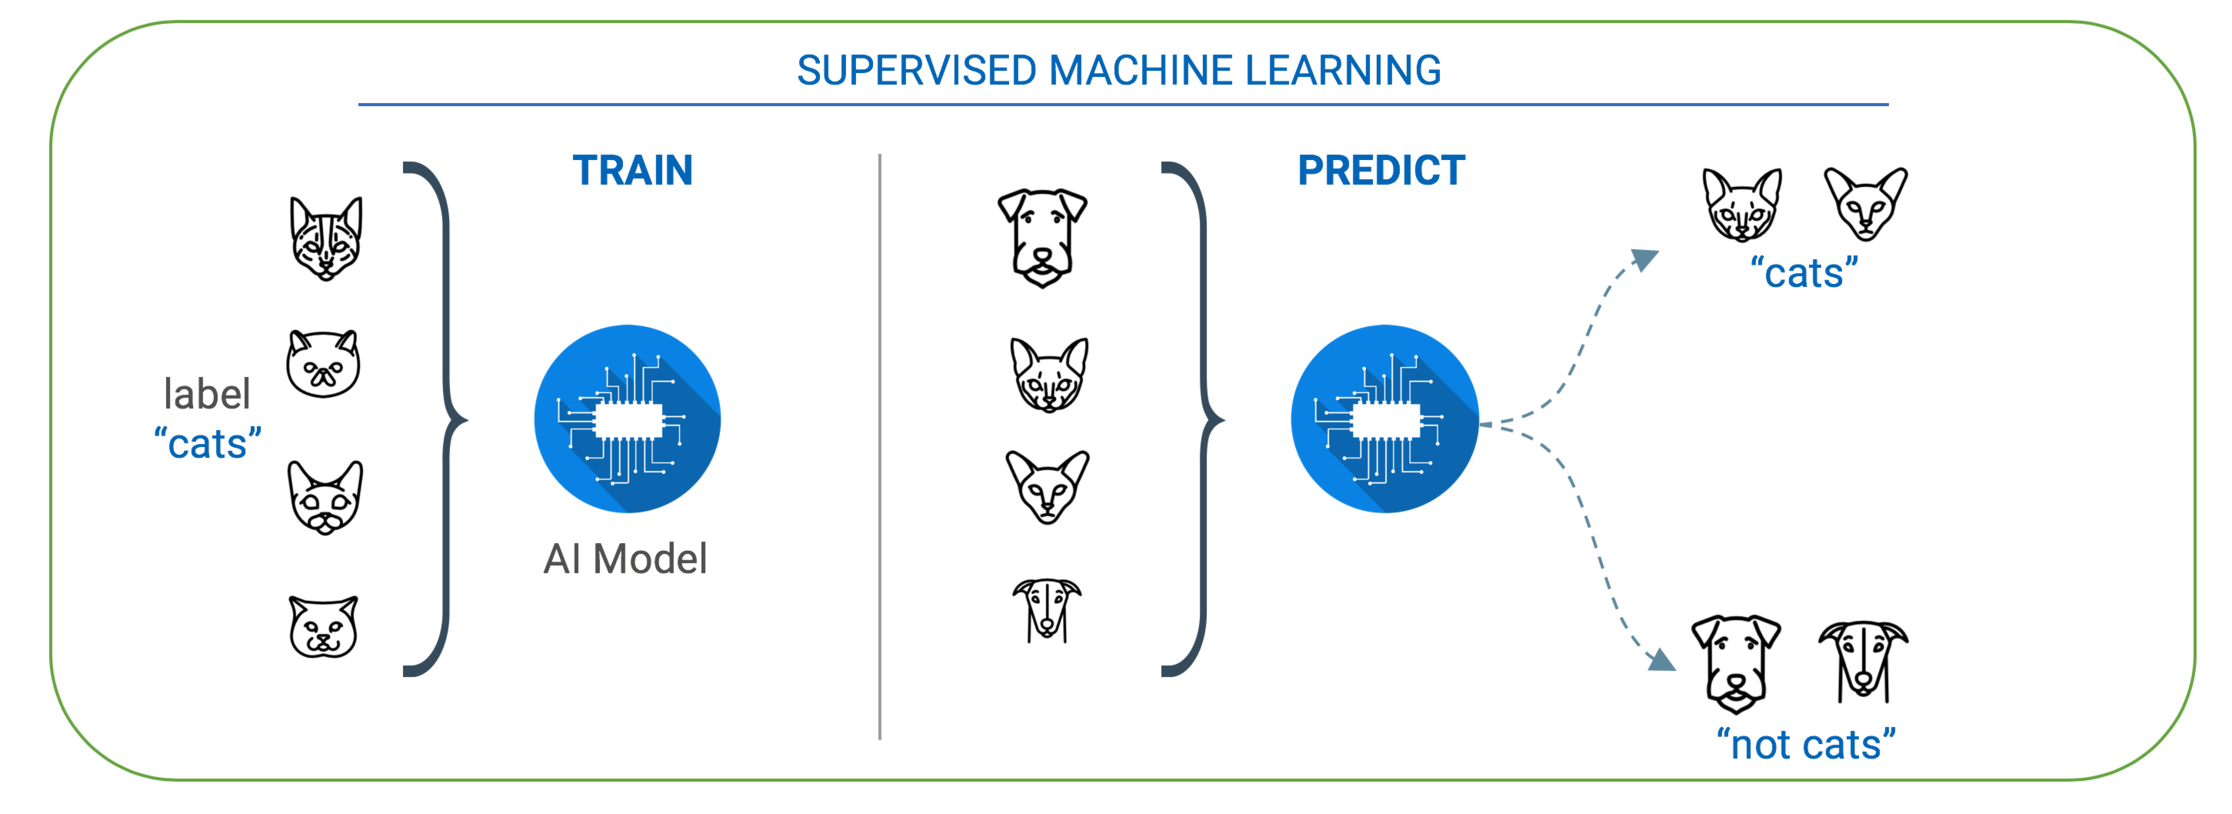
\includegraphics[width=100mm,height=40mm]{resources/supervised-machine-learning}
          };
      \end{tikzpicture}%
    \end{frame}
    
    \begin{frame}[t]{Unsupervised Machine Learning}
      \justifying It is a machine learning technique in which models are not supervised using the training dataset.in that case, it uses the hidden patterns and insights from the given data.
    
      \begin{tikzpicture}[overlay,remember picture]
        \node[anchor=south east,xshift=-40pt,yshift=25pt]
          at (current page.south east) {
            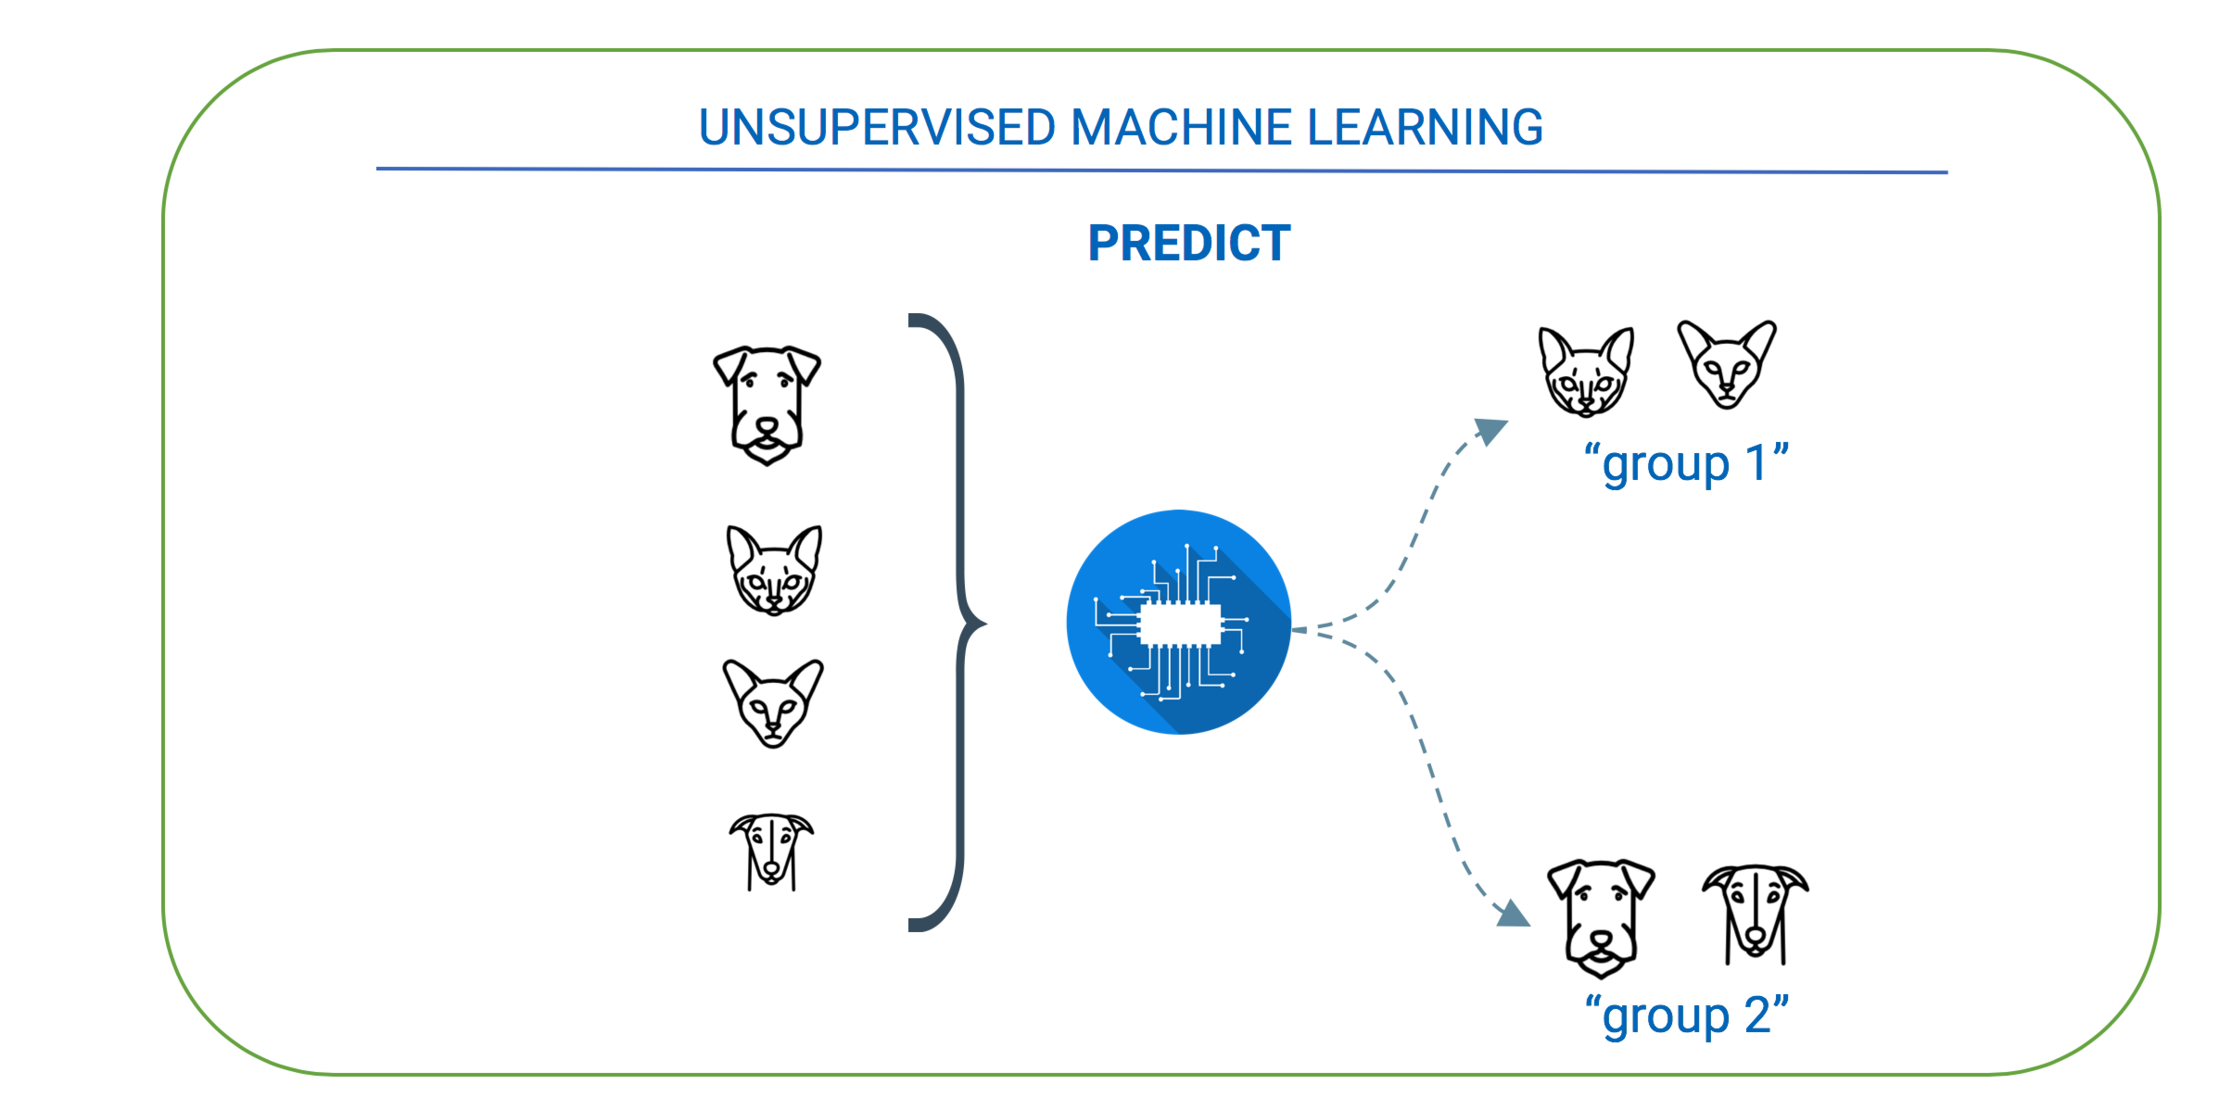
\includegraphics[width=100mm,height=40mm]{resources/unsupervied-machine-learning}
          };
      \end{tikzpicture}%
    \end{frame}
    
    \begin{frame}[t]{Semi-Supervised Machine Learning}
      \justifying It is a type of Machine Learning algorithm that comes between Supervised and Unsupervised machine learning.
      \begin{tikzpicture}[overlay,remember picture]
        \node[anchor=south east,xshift=-25pt,yshift=40pt]
          at (current page.south east) {
            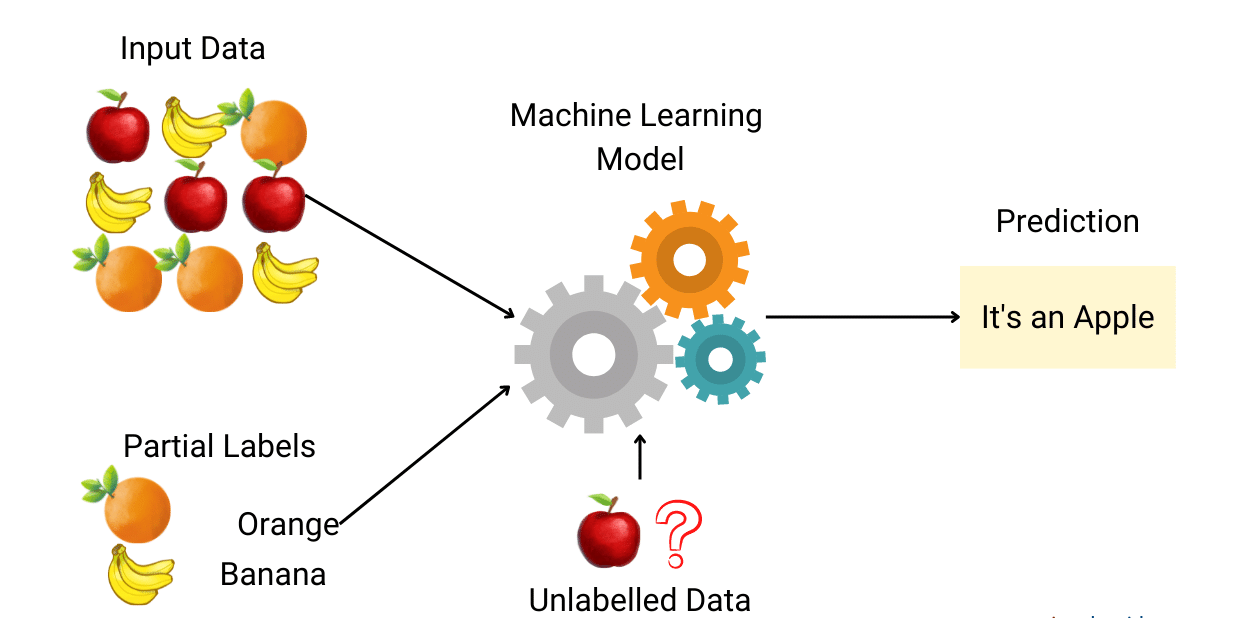
\includegraphics[width=100mm,height=40mm]{resources/semisupervised-machine-learning}
          };
      \end{tikzpicture}%
    \end{frame}

    \begin{frame}[t]{Reinforcement Learning}
      \justifying It is a type of Machine Learning that works on a feedback-based process, in which an AI agent (A software component) automatically explore its surrounding by learning from experiences, and improving its performance.
      \begin{tikzpicture}[overlay,remember picture]
        \node[anchor=south east,xshift=-50pt,yshift=10pt]
          at (current page.south east) {
            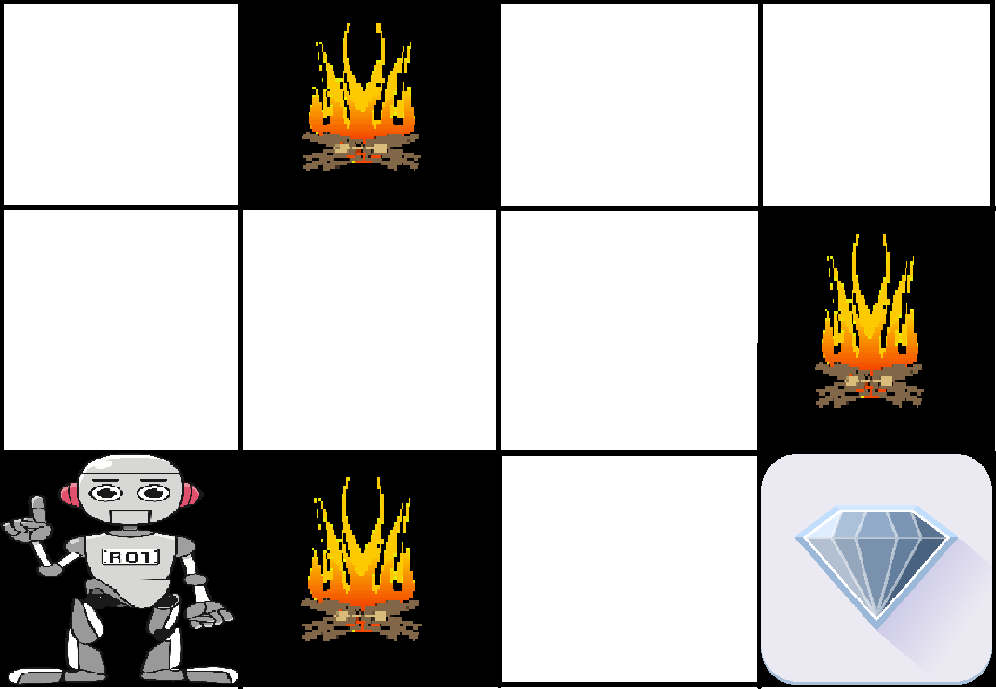
\includegraphics[width=90mm,height=45mm]{resources/reinforcement}
          };
      \end{tikzpicture}%
    \end{frame}  
    
    \begin{frame}{Artificial Intelligence Hierarchy}
        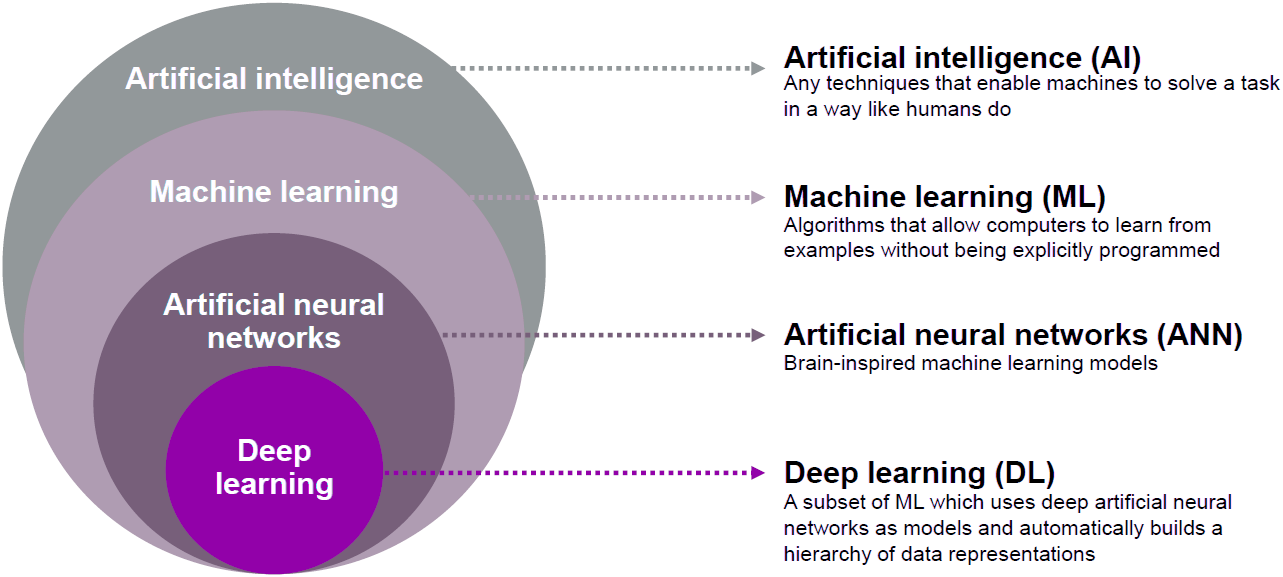
\includegraphics{resources/hierarchy}
    \end{frame}

    \subsection{Deep Learning}
    
    \begin{frame}[t]{Representation Learning}
      \framesubtitle{find best representation of our data}%
      \begin{tikzpicture}[overlay,remember picture]
        \node[anchor=south east,xshift=-30pt,yshift=35pt]
          at (current page.south east) {
            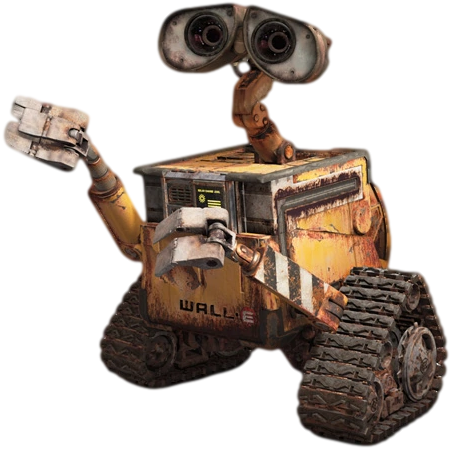
\includegraphics[width=35mm]{resources/wall-e}
          };
      \end{tikzpicture}%
      \begin{quote}
        field of study that gives computers the ability to learn without being explicitly programmed.
        \hfill {\tiny —Arthur Samuel, 1959}
      \end{quote}
      Machine Learning is the science (and art) of programming computers so they can \textit{learn from data}. \\
      \vspace{8mm}
      \parbox{0.55\textwidth}{
      Your spam filter is a Machine Learning program that, given examples of spam emails and examples of regular emails, can learn to flag spam.
      }
    \end{frame}

    \begin{frame}[t]{Deep Learning}
      \framesubtitle{a slightly general definition}%
      \begin{tikzpicture}[overlay,remember picture]
        \node[anchor=south east,xshift=-30pt,yshift=35pt]
          at (current page.south east) {
            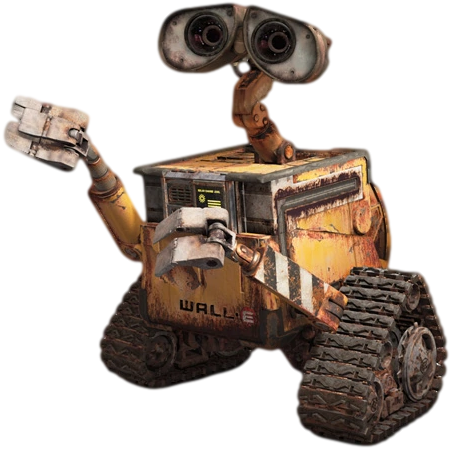
\includegraphics[width=35mm]{resources/wall-e}
          };
      \end{tikzpicture}%
      \begin{quote}
        field of study that gives computers the ability to learn without being explicitly programmed.
        \hfill {\tiny —Arthur Samuel, 1959}
      \end{quote}
      Machine Learning is the science (and art) of programming computers so they can \textit{learn from data}. \\
      \vspace{8mm}
      \parbox{0.55\textwidth}{
      Your spam filter is a Machine Learning program that, given examples of spam emails and examples of regular emails, can learn to flag spam.
      }
    \end{frame}

    \subsection{Convolutional Neural Networks}
    \begin{frame}[label=citations]{Citations}
      \framesubtitle{\TeX, \LaTeX, and Beamer}
    \end{frame}

    \section{Cancers}
    \subsection{What Is Cancer ?!}
    \begin{frame}{What Is Cancer ?} 
      \centering
      Cancer is a disease in which some of the body’s cells grow uncontrollably and spread to other parts of the body. 
      You are made up of trillions of cells that over your lifetime normally grow and divide as needed. When cells are abnormal or get old, they usually die. Cancer starts when something goes wrong in this process.
      \vfill
      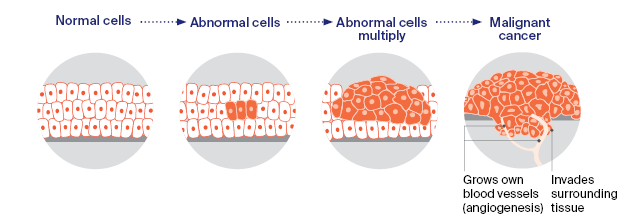
\includegraphics[height=3.5cm]{resources/How_cancer_starts}
    \end{frame}
    \subsection{Types of Cancers}

\begin{frame}{Types of Cancers}
  \framesubtitle{an overview of four major types of cancer}
  \begin{itemize}
    \item Carcinomas, a malignancy that develops from epithelial cells.
    \item Sarcomas, a malignant tumor.
    \item Leukemias, a group of blood cancers.
          \begin{itemize}
            \item Acute Lyphoblastic Leukemia
          \end{itemize}
    \item Lymphomas, a group of blood and lymph tumors.
  \end{itemize}
  \vfill
  \hfill 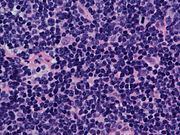
\includegraphics[width=25mm,height=20mm]{resources/lymphomas}
  \hfill 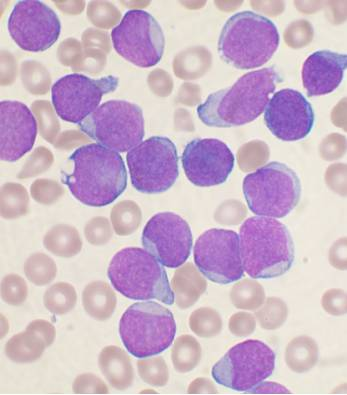
\includegraphics[width=25mm,height=20mm]{resources/leukemias}
  \hfill 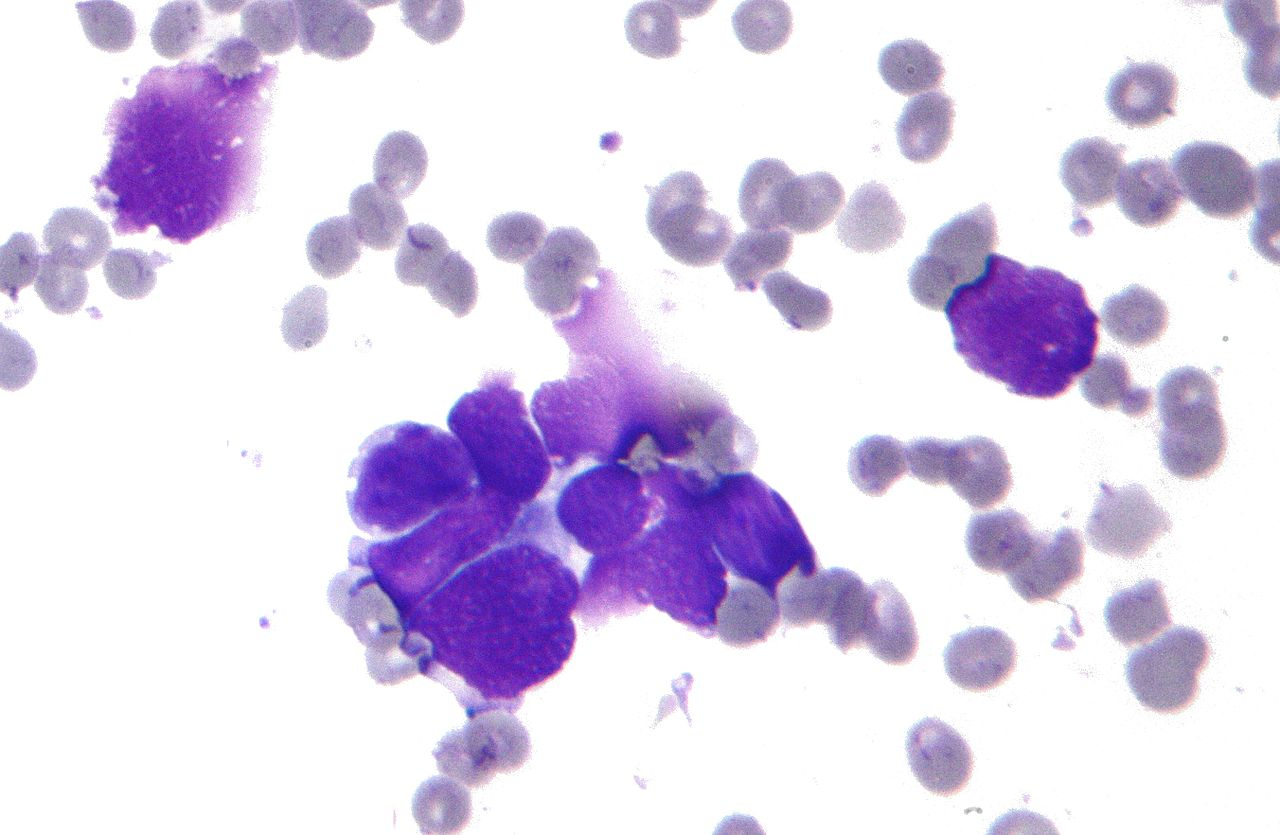
\includegraphics[width=25mm,height=20mm]{resources/carincomas}
  \hfill 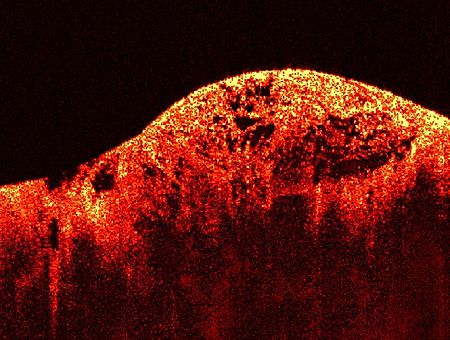
\includegraphics[width=25mm,height=20mm]{resources/sarcomas}
  \hfill

\end{frame}
    \begin{frame}[label=all]{Acute Lymphoblastic Leukemia}
      \begin{columns}
        \begin{column}{0.5\textwidth}
          Acute lymphocytic leukemia (ALL) is a type of cancer 
          of the blood and bone marrow, where blood cells are made. \\
           Normal lymphoblasts develop into mature, B-cells or T-cells.
           In ALL, both the normal development of some 
           lymphocytes and the control over the number of 
           lymphoid cells become defective.
        \end{column}
        \begin{column}{0.4\textwidth}
          \begin{figure}
            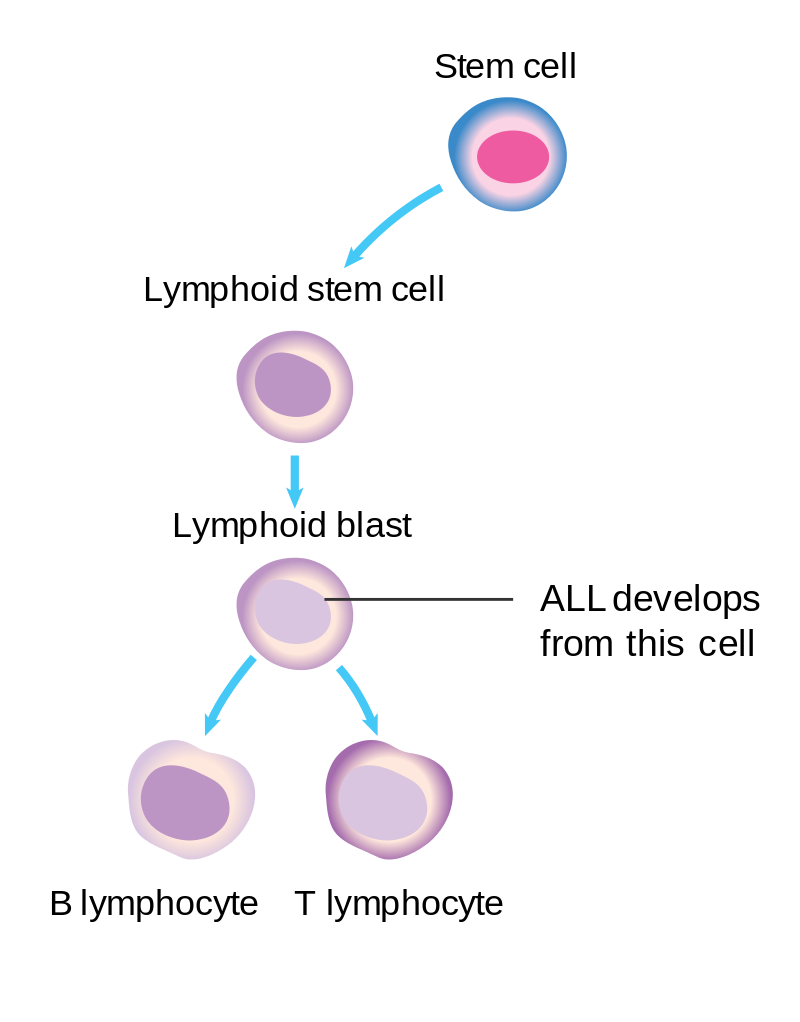
\includegraphics[width=\textwidth]{resources/all.png}
          \end{figure}
        \end{column}
      \end{columns}
    \end{frame}

    \section{Deep Learning Revisited: Cancer Detection}
    \subsection{Traditional Cancer Detection}
    \begin{frame}[t]{Cancer Detection}
      \framesubtitle{how cancer is diagnosed}%
      \begin{tikzpicture}[overlay,remember picture]
        \node[anchor=south east,xshift=-30pt,yshift=35pt]
          at (current page.south east) {
            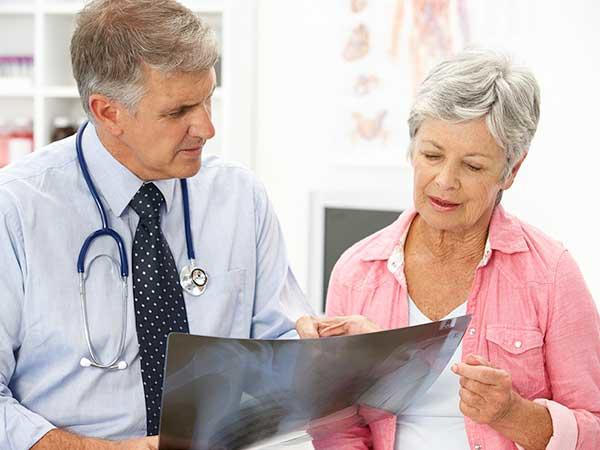
\includegraphics[width=40mm]{resources/male-doctor-elderly-female-patient-article}
          };
      \end{tikzpicture}%
      \begin{quote}
        Diagnosing cancer at its earliest stages often provides the best chance for a cure.
      \end{quote}
      If you have a symptom or a screening test result that suggests cancer, 
      your doctor must find out whether it is due to cancer or some other cause. \\ 
      \vspace{5mm}
      \parbox{0.55\textwidth}{
        The doctor may start by asking about your personal 
        and family medical history and do a physical exam. 
        The doctor also may order lab tests, imaging tests, 
        or other tests or procedures.
      }
    \end{frame}
    \subsection{Machine Learning for Cancer Detection}
    \begin{frame}[t]{Cancer Detection}
      \framesubtitle{can AI help see cancer in new, and better, ways ?}
      AI could make image interpretation—a highly subjective task—more straightforward and reliable. \\
      AI algorithms may pick up on patterns that are not readily discernable to the human eye or brain. \\
      AI can automate assessments and tasks that humans currently can do, but \textbf{take a lot of time},
      After the AI gives a result, a doctor simply needs to review what the AI has done. \\
      \vfill
      \centering
      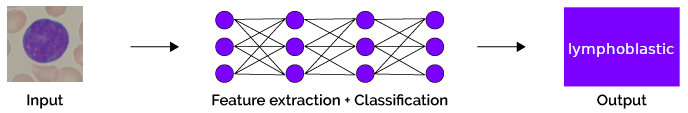
\includegraphics[height=18mm]{resources/lymphblastic-dl}
    \end{frame}
    \subsection{Practical Example}
    \begin{frame}[t]{Practical Example}
      \framesubtitle{ALL detection using tensorflow \& keras}
      TensorFlow is a free and open-source software library for machine learning and artificial intelligence. \\
        Snippets:\\ \small\href{https://colab.research.google.com/drive/10HxVDW6xJhsRg3Reog5af3Hu5kKQWuju}{colab.research.google.com/drive/10HxVDW6xJhsRg3Reog5af3Hu5kKQWuju}
        Dataset:\\ \small\href{https://www.kaggle.com/datasets/nikhilsharma00/leukemia-dataset}{www.kaggle.com/datasets/nikhilsharma00/leukemia-dataset}
      \begin{columns}
        \begin{column}{0.5\textwidth}
          \begin{figure}
            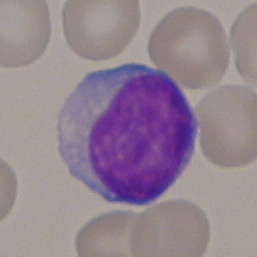
\includegraphics[height=2cm]{resources/Im166_0}
            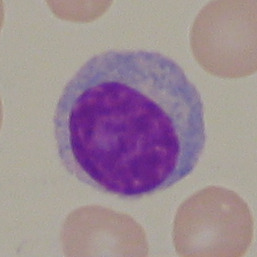
\includegraphics[height=2cm]{resources/Im196_0}
            \caption{Normal Cells}
          \end{figure}
        \end{column}
        \begin{column}{0.5\textwidth}
          \begin{figure}
            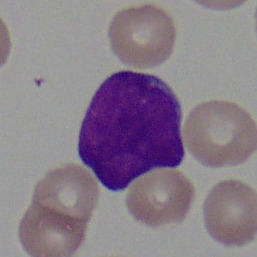
\includegraphics[height=2cm]{resources/Im063_1}
            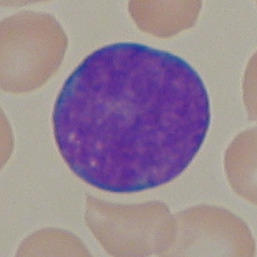
\includegraphics[height=2cm]{resources/Im129_1}
            \caption{Cancer Cells}
          \end{figure}
        \end{column}
      \end{columns}
    \end{frame}
    \subsection{In Real Life}
    \begin{frame}{In Real Life}
      \framesubtitle{are AI tools for cancer imaging ready for the real world ?}
      Over the past several years, researchers have developed AI tools that have the potential to make cancer imaging faster, more accurate, and even more informative. And that’s generated a lot of excitement. \\
      AI-based computer programs have been used to help doctors interpret mammograms for more than 20 years, but research in this area is quickly evolving. \\
      Although scientists are churning out AI tools for cancer imaging, the field is still nascent and many questions about the practical applications of these tools remain unanswered. \\
    \end{frame}

\begin{frame}[label=bibliography]{Bibliography}
  \framesubtitle{\TeX, \LaTeX, and Beamer}
  \begin{thebibliography}{9}
    \bibitem{wikipedia}
    The free encyclopedia at
    \href{https://wikipedia.org}{wikipedia.org}
    \bibitem{handson}
    Hands-On Machine Learning with Scikit-Learn and TensorFlow: Concepts, Tools, and Techniques to Build Intelligent Systems
    \bibitem{dlb}
    Deep Learning (Ian J. Goodfellow, Yoshua Bengio and Aaron Courville), MIT Press, 2016.
    \bibitem{dlp}
    Deep Learning with Python (Francois Chollet), Manning Publications, 2017.
    \bibitem{cgov}
    National Cancer Institute, \href{https://www.cancer.gov}{www.cancer.gov}
    \bibitem{mayo}
    Mayo Clinic, \href{https://www.mayoclinic.org}{www.mayoclinic.org}
  \end{thebibliography}
\end{frame}

\end{document}
